\documentclass[tikz,border=2pt]{standalone}
\usepackage{xcolor}
\definecolor{forestgreen}{rgb}{0.0,0.5,0.0}

\begin{document}
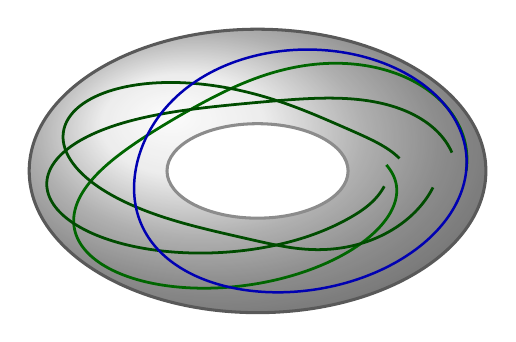
\begin{tikzpicture}[scale=1]
  \def\R{2.1}
  \def\r{0.55}
  \pgfmathdeclarefunction{torusX}{2}{%
    \pgfmathparse{(\R + \r*cos(#2))*cos(#1) + 0.35*\r*sin(#2)}%
  }
  \pgfmathdeclarefunction{torusY}{2}{%
    \pgfmathparse{0.6*(\R + \r*cos(#2))*sin(#1) + 0.45*\r*sin(#2)}%
  }

  \shade[ball color=gray!25,opacity=0.8] (0,0) ellipse (2.9 and 1.8);
  \fill[white] (0,0) ellipse (1.15 and 0.6);
  \draw[line width=1.1pt,black!65] (0,0) ellipse (2.9 and 1.8);
  \draw[line width=1.1pt,black!45] (0,0) ellipse (1.15 and 0.6);

  \def\alpha{1.45}
  \foreach \shift/\col in {0/forestgreen!80!black,70/forestgreen!60!black,140/forestgreen!60!black}{
    \draw[\col,line width=1pt,samples=240,smooth,domain=0:360,variable=\u]
      plot ({torusX(\u,\alpha*\u+\shift)},{torusY(\u,\alpha*\u+\shift)});
  }
  \draw[blue!70!black,line width=0.9pt,samples=200,smooth,domain=0:360,variable=\u]
    plot ({torusX(\u,\u)},{torusY(\u,\u)});
\end{tikzpicture}
\end{document}
